Для адекватного моделирования уравнения переноса
\[ \frac{\partial f}{\partial t} + \xi_i\frac{\partial f}{\partial X_i} = 0 \]
с произвольными начальными условиями \( f(t=0)\)
необходимо сочетание \textit{консервативности}, \textit{монотонности} и \textit{сходимости} разностной схемы.
Этого легко добиться при первом порядке аппроксимации,
однако в таком случае требуются достаточно подробные разностные сетки для достижения высокой точности.
Кроме того, так называемая \textit{схемная вязкость} значительным образом <<размывает>> решение со временем.
Для достижения высоких порядков аппроксимации, приходится строить \textit{нелинейные} разностные схемы.
Историю развития разностных схем для решения гиперболических уравнений можно найти в \cite{vanLeer2006}.

\subsubsection{Сравнение расностных схем}

При поиске оптимальной разностной схемы рассмотрены два подхода.
Первый подход основан на \textit{методе коррекции потоков} (\textit{Flux-Corrected Transport}),
впервые описанный в 1973 году Джеем Борисом (Jay Boris) и Дэвидом Буком (David Book)~\cite{Boris1973},
имеющий структуру предиктор-корректор.
Для простоты рассмотрим одномерную прямоугольную сетку с ячейками размером \(h\),
на которой эволюционирует с временн\textit{ы}м шагом \(\tau\) разностная функция \(f_i^n = f(x_i,t_n)\).
С помощью интегро-интерпо\-ляционного метода~\cite{Samarsky1961} получается консервативная разностная схема второго порядка точности:
\begin{gather}\label{eq:pk}
	f_i^{n+1} = f_i^n - \gamma(f_{i+1/2}^{n+1/2}-f_{i-1/2}^{n+1/2}), \\
	f_{i+1/2}^{n+1/2} \equiv f\left(x_i+\frac{h}{2},t_n+\frac{\tau}{2}\right)+\mathcal{O}(h^2,\tau^2)
	= f_i^n + \frac{1-\gamma}{2}\varphi(\theta_i^n)(f_{i+1}^n - f_i^n),
\end{gather}
где \[ \gamma=\frac{\xi\tau}{h}, \; \theta_i = \frac{f_i - f_{i-1}}{f_{i+1} - f_i} = 1-h\frac{f_{xx}}{f_x}+\mathcal{O}(h^2).\]
Постоянная \(\gamma\) "--- \textit{число Куранта} (\textit{Courant"--~Friedrichs"--~Lewy}).
Шаблон такой разностной схемы представлен на рис.~\ref{fig:pattern}
Функция \(\varphi(\theta)\) называется ограничителем (англ. \textit{limiter}),
её аргумент \(\theta\) "--- показателем гладкости решения.

Можно предложить наглядную геометрическую интерпретацию ограничителей
на основе алгоритма \textit{REA} (\textit{reconstruct-evolve-average}) [].
Для этого используем кусочно-линейную аппроксимацию разностной функции (рис.~\ref{fig:piecewise}):
\[ f(x,t_n) = f_i^n + \sigma_i^n (x-x_i), \]
тогда разностная схема примет вид \eqref{eq:pk}, где
\[ \varphi(\theta_i^n) = h\sigma_i^n. \]
Таким образом, ограничитель определяет наклон аппроксимации разностной функции в ячейке.
Для схемы первого порядка \(\sigma_i^n=0\).

\begin{figure}
	\centering
	\subfloat[шаблон разностной схемы]{\label{fig:pattern}
		\begin{tikzpicture}[point/.style={shape=circle,draw,fill,minimum size=2mm,inner sep=0,node distance=2cm},
							red/.style={thin,color=red,->}, blue/.style={thin,color=blue,->},
							>=latex', thick, scale=1.5]
			\node[point] (30) at (-2,0) {}; \node[below] at (30.south) {\(f_{i-2}^n\)};
			\node[point] (20) at (1,0) {}; \node[below] at (20.south) {\(f_{i+1}^n\)};
			\node[point] (10) at (0,0) {}; \node[below] at (10.south) {\(f_i^n\)};
			\node[point] (00) at (-1,0) {}; \node[below] at (00.south) {\(f_{i-1}^n\)};
			\node[point] (11) at (0,1) {}; \node[above] at (11.north) {\(f_i^{n+1}\)};
			\node[red] (l) at (-.5,.5) {\(\times\)};
			\node[blue] (r) at (.5,.5) {\(\times\)};
			\node[above left] at (l) {\(f_{i-1/2}^{n+1/2}\)};
			\node[above right] at (r) {\(f_{i+1/2}^{n+1/2}\)};
			\draw[-] (10) to (00); \draw[-] (10) to (20); \draw[-] (10) to (30); \draw[-] (10) to (11);
			\draw[red] (11) to (l); \draw[red] (l) to (10); \draw[red] (l) to (00); \draw[red] (l) to (30);
			\draw[blue] (11) to (r); \draw[blue] (r) to (10); \draw[blue] (r) to (00); \draw[blue] (r) to (20);
		\end{tikzpicture}}
	\quad\quad
	\subfloat[кусочно-линейная аппроксимация]{\label{fig:piecewise}
			\begin{tikzpicture}[point/.style={shape=circle,draw,fill,minimum size=2mm,inner sep=0, node distance=2cm},
								back/.style={draw=gray!20,fill=gray!20}, >=latex', very thick, scale=1]
				\draw[back] (.5,-1) -- (.5,-.2) -- (1.5,.2) -- (1.5,-1) -- cycle;
				\draw[back] (1.5,-1) -- (1.5,0) -- (2.5,2) -- (2.5,-1) -- cycle;
				\draw[back] (2.5,-1) -- (2.5,2.4) -- (3.5,2.6) -- (3.5,-1) -- cycle;
				\draw[back] (3.5,-1) -- (3.5,2.4) -- (4.5,1.6) -- (4.5,-1) -- cycle;
				\node[point] (p1) at (1,0) {}; \node[point] (p2) at (2,1) {}; \node[point] (p3) at (3,2.5) {}; \node[point] (p4) at (4,2) {};
				\draw[-] (.5,-.2) to (1.5,.2); \draw[-] (1.5,0) to (2.5,2); \draw[-] (2.5,2.4) to (3.5,2.6); \draw[-] (3.5,2.4) to (4.5,1.6);
				\foreach \x in {0.5,1.5,2.5,3.5,4.5} \draw[dashed] (\x,-1) to (\x,3);
			\end{tikzpicture}}
\end{figure}

Другой подход "--- это интерполяция \(\partial f/\partial x\) также по потоковой схеме
\begin{equation}\label{eq:rk1}
	L(f_i) = - \frac{\xi}{h}(f_{i+1/2}-f_{i-1/2}),\;
	f_{i+1/2} = f_i + \frac1{2}\varphi(\theta_i)(f_{i+1} - f_i),
\end{equation}
и использование методов Рунге"--~Кутты для решения задачи Коши:
\begin{equation}\label{eq:rk2}
	\partial f/\partial t = L(f).
\end{equation}

Обе схемы устойчивы при \(\gamma < 1\) (мы рассматриваем только положительные значения скорости,
поскольку для отрицательных формулы получаются симметричным отражением).

\begin{wraptable}{r}{5cm}
	\vspace{-10pt}
	\caption{Бутчера для схемы Хойна}\label{tab:bootcher}
	\vspace{-10pt}
	\centering
		\begin{tabular}{| c | c | c | c |}
			\hline
			0 & & & \\ \hline
			\(1/3\) & \(1/3\) & & \\ \hline
			\(2/3\) & 0 & \(2/3\) & \\ \hline
			& \(1/4\) & 0 & \(3/4\) \\ \hline
		\end{tabular}
	\vspace{-10pt}
\end{wraptable}

Сравнивались лимитеры, перечисленные в табл.~\ref{tab:limiters} и изображенные на диаграмме Свеби (Sweby)~\cite{Sweby1984} (рис.~\ref{fig:sweby}). 
Нулевому лимитеру соответствует \textit{схема первого порядка} точности (\textit{upwind}).
Невязка, содержащая вторую произодную \(f_{xx}\), называется диффузной, поскольку аппроксимирует уравнение диффузии,
которое вызывает размытие решения во времени. Для борьбы с этим вводят так называемые \textit{антидиффузионные} потоки,
которые соответствуют положительному ограничителю \(\varphi(\theta)>0\).
Для второго порядка аппроксимации по методу \eqref{eq:pk} необходимо
\[ \lim_{\theta\to1}{\varphi(\theta)} = 1, \; \exists \lim_{\theta\to1}{\varphi'(\theta)}. \]
Непрерывность производной обеспечивает второй порядок точности около точек перегиба,
поскольку в этом случае происходит переход через точку \(\theta=1\).

Прямые на рис.~\ref{fig:sweby:a}, проходящие через точку (1,1), соответствуют классическим разностным схемам
Лакса"--~Вендроффа (Lax"--~Wendroff)~\cite{Lax1960}, Фромма (Fromm) ~\cite{Fromm1968} и Бима"--~Уорминга (Beam"--~Warming)~\cite{Warming1975}.
Схема Лакса"--~Вендроффа для корректировки потоков использует значение функции в следующей по направлению скорости ячейке
(англ. \textit{upwind}), Схема Бима"--~Уорминга, напротив, "--- с предыдущей ячейки (англ. \textit{downwind}).
Схема Фромма симметрична в этом отношении, что приводит к обнулению коэффициента перед третьей производной.

Согласно теореме Годунова эти линейные схемы теряют свойство монотонности, столь необходимое в решениях с большими градиентами.
Это приводит, во-первых, к возникновению \textit{паразитических осцилляций} на разрывных решениях,
во-вторых, к \textit{фазовому сдвигу} (за исключением схемы Фромма) быстро осциллирующих решений.
Всё это объясняется неограниченными членами, аппроксимирующими старшие производные.

\begin{table}
	\centering\caption{Список лимитеров.}\label{tab:limiters}
	\begin{tabular}{p{1cm}cc}
		& Название			&  Лимитер \( \varphi(\theta) \) \smallskip \\
		\hline \noalign{\smallskip}
		\multirow{4}{*}{\rotatebox{90}{\parbox{2.7cm}{\centering\footnotesize Классические схемы}}}
		& первый порядок	& \( 0 \) \smallskip \\
		& Лакс"--~Вендрофф	& \( 1 \) \smallskip \\
		& Фромм				& \( \dfrac{1+\theta}2 \) \smallskip \\
		& Бим"--~Уорминг	& \( \theta \) \smallskip \\
		\hline \noalign{\smallskip}
		\multirow{6}{*}{\rotatebox{90}{\parbox{5.5cm}{\centering\footnotesize TVD схемы \( \varphi(\theta<0)=0 \)}}}
		& \textit{minmod}			& \( \min\left(\theta,1\right) \) \smallskip \\
		& \textit{MC} 				& \( \min\left(2\theta,\dfrac{1+\theta}{2},2\right) \) \smallskip \\
		& \textit{Koren} 			& \( \min\left(2\theta,\dfrac{2+\theta}{3},2\right) \) \smallskip \\
		& \textit{superbee}		 	& \( \max(\min(2\theta,1),\min(\theta,2)) \) \smallskip \\
		\cline{2-3} \noalign{\smallskip}
		& \textit{wide superbee} 	& \( \max\left(\min\left(\dfrac2{\gamma}\theta,1\right),\min\left(\theta,\dfrac2{1-\gamma}\right)\right) \) \smallskip \\
		& \textit{wide third}		& \( \min\left(\dfrac2{\gamma}\theta,\dfrac{(\gamma+1)\theta+(2-\gamma)}{3},\dfrac2{1-\gamma}\right) \) \smallskip \\
		\hline \noalign{\smallskip}
	\end{tabular}
\end{table}

\begin{figure}
	\footnotesize
	\subfloat[классические схемы]{\label{fig:sweby:a}
		\begin{tikzpicture}[>=latex',thick, scale=1.5, domain=0:4]
			\draw[draw=gray!20,fill=gray!20] (0,0) -- (1,2) -- (4.1,2) -- (4.1,0) -- cycle;
			\node[above] at (.8,0) {TVD};
			\draw[<->] (4.2,0) node[right] {\(\theta\)} -- (0,0) -- (0,2.7) node[above] {\(\varphi(\theta)\)};
			\foreach \x in {0,1,2,3,4}
				\draw (\x cm,1pt) -- (\x cm,-1pt) node[anchor=north] {\(\x\)};
			\foreach \y in {0,1,2}
				\draw (1pt,\y cm) -- (-1pt,\y cm) node[anchor=east] {\(\y\)};
			\node[draw,circle,minimum size=.3cm] (sec) at (1,1) {};
			\node[text width=1.5cm,text centered] (cap) at (0.8,1.7) {второй\vspace{-4pt} порядок};
			\draw[->] (cap.south) to (sec);

			\draw[color=purple!50!blue] (0,0) -- (0.25,0.5) -- (2.5,2) -- (2.7,2) node[above] {\textit{Koren}} -- (4,2);
			\draw[color=green!50!black] (0,0) -- (0.333,0.667) -- (3,2) node[below right] {\textit{MC}} -- (4,2);
			\draw[color=blue] (-.1,-.1) -- (2.2,2.2) node[above left] {Бим"--~Уорминг} -- (2.9,2.9);
			\draw[dashed,color=green] (-.1,.45) -- (4,2.5) node[above left] {Фромм};
			\draw[color=red] (-.1,1) -- (1.8,1) node[below right] {Лакс"--~Вендрофф} -- (4,1);
		\end{tikzpicture}}
	\quad
	\subfloat[улучшенные лимитеры, зависящие от \(\gamma\)]{\label{fig:sweby:b}
		\begin{tikzpicture}[>=latex',thick, scale=1, domain=0:4]
			\draw[draw=gray!10,fill=gray!10] (0,0) -- (.5,3) -- (6.2,3) -- (6.2,0) -- cycle;
			\draw[draw=gray!20,fill=gray!20] (0,0) -- (1,2) -- (6.2,2) -- (6.2,0) -- cycle;
			\node[below] at (1.5,3) {TVD \(\gamma=\frac1{3}\)};
			\node[above] at (1,0) {TVD \(\forall\gamma\)};
			\draw[<->] (6.3,0) node[right] {\(\theta\)} -- (0,0) -- (0,3.5) node[above] {\(\varphi(\theta)\)};
			\foreach \x in {0,1,2,3,4,5,6}
				\draw (\x cm,1pt) -- (\x cm,-1pt) node[anchor=north] {\(\x\)};
			\foreach \y in {0,1,2,3}
				\draw (1pt,\y cm) -- (-1pt,\y cm) node[anchor=east] {\(\y\)};
			\node[draw,circle,minimum size=.3cm] (sec) at (1,1) {};
			\node[text width=1.5cm,text centered] (cap) at (3,.8) {второй\vspace{-4pt} порядок};
			\draw[->] (cap.west) to (sec);

			\draw[color=red] (0,0) -- (.1666,1) -- (1,1) -- (3,3) -- (4,3) node[above] {\textit{wide superbee} (\(\gamma={}^1/_3\))} -- (6,3);
			\draw[color=blue] (0,0) -- (.1,.6) -- (3,1.888) node[below right] {\textit{wide third} (\(\gamma={}^1/_3\))} -- (5.5,3) -- (6,3);
		\end{tikzpicture}}
	\caption{Диаграмма Cвеби}\label{fig:sweby}
\end{figure}

Для борьбы с заявленными проблемами в 1983 году Амирам Хартен (Amiram Harten) ввёл понятие \textit{TVD схем}~\cite{Harten1983},
для которых справедливо
\[ \TV^{n+1}\le \TV^n, \quad \TV^n = \sum_i| f_{i+1}^n - f_i^n |, \]
что является более мягким условием, нежели монотонность схемы, однако \textit{явные TVD схемы} заведомо монотонны.
Лимитер в таком случае ограничивается следующей областью
\[ \left|\varphi(\theta)\right| \leq \mathrm{minmod}\left(\frac2{\gamma}\theta,\frac2{1-\gamma}\right), \] где
\[
\mathrm{minmod}\,(a,b) \equiv \left\{
\begin{array}{l l}
	a & \quad \text{if}\;|a|<|b| \;\text{and}\;ab>0, \\
	b & \quad \text{if}\;|b|<|a| \;\text{and}\;ab>0, \\
	0 & \quad \text{if}\;ab \leq 0,
\end{array}\right.
\]
которую будем называть \textit{расширенным} (\textit{wide}) условием TVD.
Кроме того, выделяют более узкий класс ограничителей\footnote{
	При решении классических задач гидрогазодинамики на основе уравнений Навье--Стокса приходится иметь дело с вектором макропараметров \(f\),
	поэтому ограничитель берут независимым от \(\gamma\), однако при моделировании скалярной функции распределения
	в кинетическом уравнении Больцмана, оказывается возможным использование предложенных выше улучшенных разностных схем.
}, соответствующий классическому условию TVD:
\[ \left\{
\begin{array}{l}
	\varphi(\theta\le0)=0, \\
	\varphi(\theta>0) > 0.
\end{array}\right.
\]
Отрицательные значения \(\theta\) соответствуют экстремумам, где в рамках линейной аппроксимации нельзя получить лучшее приближение, чем \(\varphi=0\).
Условие \(\varphi(\theta)>0\) создаёт антидиффузионные потоки, как было сказано ранее.
В литературе в основном встречается TVD условие, независимое от числа Куранта:
\[ \left|\varphi(\theta)\right| \leq \mathrm{minmod}(2\theta,2). \]

Лимитер \textit{minmod} назван по одноименной функции, поскольку равняется минимальной по модулю схеме Лакса"--~Вендроффа и Бима"--~Уорминга.
т.е. он выбирает минимальную корректировку среди запаздывающей и опережающей.
Основные его недостатки "--- это разрыв производной в точке \(\theta=1\) (уменьшает сходимость), и ограниченность условием \(\varphi\le1\)
(слабые антидиффузионные потоки). Лимитер MC (monotonized central-difference)~\cite{vanLeer1977}, который равен minmod\,\mbox{(Fromm, TVD)},
и \textit{Koren}~\cite{Koren1993} лишены обоих недостатков. Это так называемые \textit{наклонные ограничители} (\textit{slope-limiters}).

Однако на разрывных решениях максимального порядка сходимости достигает только \textit{superbee}~\cite{Roe1985},
который в противоположность \textit{minmod} использует максимально возможную корректировку потоков,
оставаясь в рамках второго порядка точности.

На рис.~\ref{fig:sweby:b} показаны лимитеры, зависящие от числа Куранта. Они описаны в ~\cite{Roe1985},
но ввиду малого распространения не получили устойчивых имён.
Лимитеры с расширенной областью, где справедливо условие TVD, условимся называть \textit{wide}, например, \textit{wide superbee}.
Кроме того, использование числа Куранта в лимитере, позволяет построить лимитер третьего порядка точности \textit{wide third}.
Его центральная прямая совпадает с \textit{MC} при \(\gamma=0.5\) и с \textit{Koren} при \(\gamma=0\).

Отметим, что \textit{Koren} "--- единственный из лимитеров, который на четырехточечном шаблоне имеет третий порядок аппроксимации по пространственной переменной
(на отрезке \( \frac{2+\theta}{3} \)). Поэтому именно он используется вместе со схемой Рунге"--~Кутты 3-го порядка точности,
наименьшей невязкой среди которых обладает схема Хойна (табл.~\ref{tab:bootcher}).

\subsubsection{Исследование на сходимость}

Простейшая задача для сравнения лимитеров "--- это одномерная задача переноса с фиксированной скоростью без граничных условий.
На рис.~\ref{fig:conver} представлено поведение всех заявленных лимитеров при числе Куранта \(\gamma=0.5\) слева направо:
на гладком решении, с разрывом производной, разрывом самой функции и для быстро осциллирующего решения.

\begin{figure}
	\subfloat[схема первого порядка]{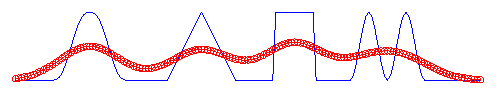
\includegraphics[width=0.5\textwidth]{limiters/first}}
	\subfloat[схема Лакса"--~Вендроффа]{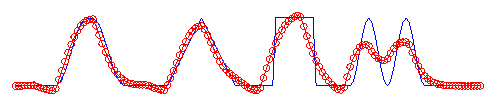
\includegraphics[width=0.5\textwidth]{limiters/lw}}\\
	\subfloat[схема Фромма]{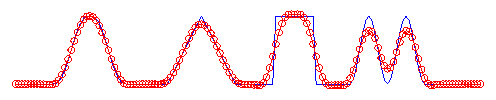
\includegraphics[width=0.5\textwidth]{limiters/fromm}}
	\subfloat[схема Бима"--~Уорминга]{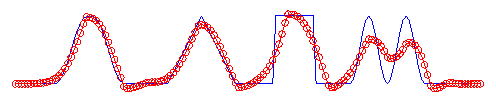
\includegraphics[width=0.5\textwidth]{limiters/bw}}\\
	\subfloat[\textit{minmod} лимитер]{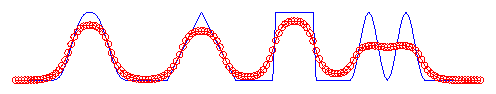
\includegraphics[width=0.5\textwidth]{limiters/minmod}}
	\subfloat[\textit{superbee} лимитер]{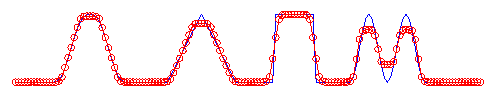
\includegraphics[width=0.5\textwidth]{limiters/superbee}}\\
	\subfloat[\textit{MC} лимитер]{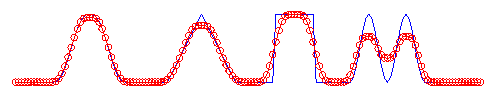
\includegraphics[width=0.5\textwidth]{limiters/mc}}
	\subfloat[\textit{wide superbee} лимитер]{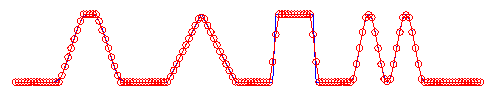
\includegraphics[width=0.5\textwidth]{limiters/superbee_g}}\\
	\subfloat[\textit{wide third} лимитер]{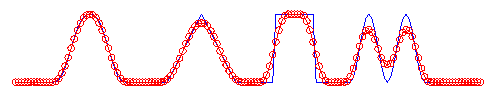
\includegraphics[width=0.5\textwidth]{limiters/third_g}}
	\subfloat[схема Хойна с лимитером Koren]{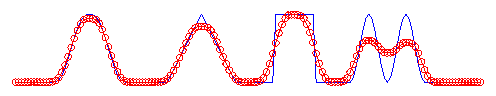
\includegraphics[width=0.5\textwidth]{limiters/runge}}\\
	\caption{Поведение различных схем при числе Куранта \(\gamma=1/2\) на различных начальных условиях:
		гладкое, разрыв первой производной, самой функции и при наличии быстрых осцилляций}\label{fig:conver}
\end{figure}

Сразу видно, что схема первого порядка даёт неудовлетворительные результаты, поскольку <<размазывает>> форму всех импульсов,
поэтому рекомендуется использовать её только для грубых качественных расчётов.
Классические схемы (особенно схема Фромма) дают неплохие результаты, однако отсутствие условия TVD влечёт за собой паразитические осцилляции,
в частности, нарушается условие неотрицательности, что особенно важно при решении кинетического уравнения,
поэтому их также стоит непригодными для использования. Отметим, что схема Фромма ввиду своей симметричности лишён фазового сдвига
по сравнению с запаздывающим решением Лакса"--~Вендроффа и опережающим Бима"--~Уорминга.

Наихудшим среди TVD лимитеров второго порядка точности, как и ожидалось, стал \textit{minmod}.
Лучше всего гладкие решения аппроксимирует \textit{MC} и \textit{wide third} лимитеры,
поскольку они (это относится и к схеме Фромма) имеют одинаковое значение производной \(\varphi'(1)\).
Отличия обуславливаются различным поведением при больших градиентах.
Видно, что \textit{wide third} лучше сходится к экстремумам функции.
Напомним, что, кроме прочего, \textit{wide third} имеет третий порядок сходимости при любых \(\gamma\) в отличие от конкурентов
(значение \(\gamma=0.5\) выбрано специально для сравнения схем третьего порядка).

В сходимости к разрывным и быстро осциллирующим решениям с большим перевесом первенствует \textit{wide superbee},
который также по всем показателям обошел своего классического <<коллегу>> \textit{superbee}.

Для численного сравнения лимитеров использовалась октаэдрическая норма:
\begin{equation}\label{eq:octahedron}
	D(M) = \|f-v\| = \frac1{M}\sum_{i=1}^{M}|f_i-v_i| = \mathcal{O}(h^q)
\end{equation}
где \(v_i\) "--- точное решение, \(h\) "--- сеточный шаг, \(q\) "--- порядок сходимости, \(M\) "--- общее число ячеек.
На гладких решениях порядок сходимости при условии сходимости совпадает с порядком аппроксимации согласно теореме Лакса"--~Рябенького.
В противном случае на сегодняшний день теоретический анализ затруднителен, поэтому будем использовать экспериментальные значения.
В табл.~\ref{tab:q_value} представлены соответствующие значения порядков сходимости исследуемых схем 
для разрывных и гладких функций при \(\gamma=0.9\). Они вычислялись по простой формуле
\[ q = \log_2\frac{D(M)}{D(2M)}. \]
Аналогичное сравнение широкого класса численных схем можно найти в \cite{Safronov2010}.

\begin{table}
	\caption{Порядки сходимости исследуемых схем}\label{tab:q_value}
	\centering
	\begin{tabular}{l|c|c}
		\multirow{3}{*}{\bf схема/лимитер} & \multicolumn{2}{c}{\bf порядок сходимости} \\ \cline{2-3}
								& \multicolumn{2}{c}{тип функции} \\ \cline{2-3}
								& разрывная & гладкая \\ \hline
		первого порядка			& 0.500 	& 0.997 \\ \hline
		Лакса"--~Вендроффа		& 0.582 	& 1.999 \\ \hline
		\textit{minmod}			& 0.658 	& 1.990 \\ \hline
		\textit{MC}				& 0.691 	& 2.000 \\ \hline
		\textit{superbee}		& \color{olive}0.997 & 2.000 \\ \hline
		\textit{wide superbee}	& \color{olive}1.000 & 2.000 \\ \hline
		\textit{wide third}		& 0.747 	& \color{magenta}2.947 \\ \hline
		Хойна + \textit{Koren}	& 0.751 	& \color{magenta}2.899
	\end{tabular}
\end{table}

\begin{figure}
	\centering
	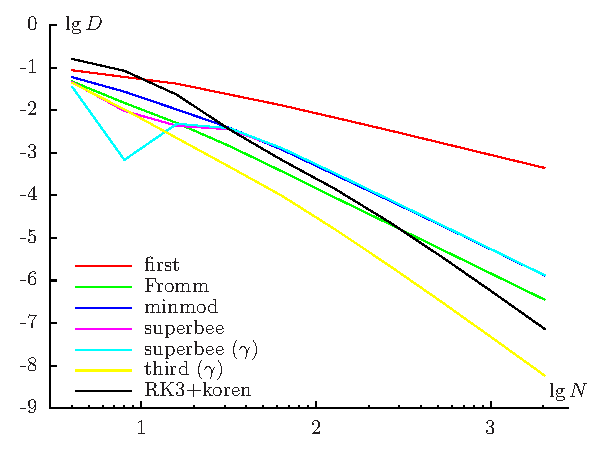
\includegraphics[width=.8\textwidth]{limiters/residual}
	\caption{Зависимость невязки от мелкости сетки}\label{fig:residual}
\end{figure}

Схема первого порядка теряет свой порядок только на разрывных решений,
где значение \(q=0.5\) объясняется схемной вязкостью (см. приложение в []).
Остальные схемы отчетливо проявили свой порядок на гладком решении,
поэтому в таких случаях предпочтение стоит отдать схемам третьего порядка \textit{wide third} и схеме Хойна с лимитером \textit{Koren}.
Стоит однако отметить, что использование схем Рунге"--~Кутты требует в несколько раз б\textit{о}льших вычислительных затрат.

Что касается разрывных решений, то максимальный порядок (\(q=1\)) продемострировали \textit{superbee} и \textit{wide superbee}.
Выделение класса схем с единичным порядком "--- сложная задача, но, по-видимому,
\textit{superbee} схемы представляют собой наилучшее сочетание со вторым порядком аппроксимации.

Кроме порядка сходимости особый интерес представляет также абсолютное значение невязки.
На рис.~\ref{fig:residual} показана зависимость невязки от количества ячеек \(N\), приходящихся на ненулевое значение \(f(0,x)\).
На гладких функциях, как и предполагалось, наименьшую невязку на мелких сетках показал \textit{wide third},
однако на грубых сетках благодаря большим антидиффузионным потокам отличный результат показывает \textit{wide superbee}.

\subsubsection{Резюме}

В результате проведённого исследования (подробнее см. в []) можно выделить две наилучшие схемы:
это схемы с коррекцией потоков на основе ограничителей \textit{wide superbee} и \textit{wide third}.
Первый из них обладает максимальным порядком сходимости на разрывных решениях (единица в октаэдрической норме \eqref{eq:octahedron}).
Кроме того, он рекомендуется при использовании грубых разностных сеток и для быстроосциллирующих решений.
Второй на гладких решениях показывает максимально возможный (на пятиточечном разностном шаблоне) третий порядок сходимости,
что определяет его применимость для прецизионных вычислений.
